% This version of CVPR template is provided by Ming-Ming Cheng.
% Please leave an issue if you found a bug:
% https://github.com/MCG-NKU/CVPR_Template.

%\documentclass[review]{cvpr}
\documentclass[final]{cvpr}

\usepackage{times}
\usepackage{epsfig}
\usepackage{graphicx}
\usepackage{amsmath}
\usepackage{amssymb}
\usepackage{mathtools}
\usepackage{float}
\usepackage[table,xcdraw]{xcolor}
\usepackage{comment}

\usepackage{biblatex} %Imports biblatex package
\addbibresource{references.bib}

% Include other packages here, before hyperref.

% If you comment hyperref and then uncomment it, you should delete
% egpaper.aux before re-running latex.  (Or just hit 'q' on the first latex
% run, let it finish, and you should be clear).
\usepackage[pagebackref=true,breaklinks=true,colorlinks,bookmarks=false]{hyperref}


\def\cvprPaperID{****} % *** Enter the CVPR Paper ID here
\def\confYear{MVA 2022}
%\setcounter{page}{4321} % For final version only


\begin{document}

%%%%%%%%% TITLE
\title{Cellular Component Ontology Prediction \\ \small{Final project report - JMA team - MVA ALTeGraD course}}

\author{Jérémie Dentan\\
École Polytechnique\\
{\tt\small jeremie.dentan@polytechnique.org}
% For a paper whose authors are all at the same institution,
% omit the following lines up until the closing ``}''.
% Additional authors and addresses can be added with ``\and'',
% just like the second author.
% To save space, use either the email address or home page, not both
\and
Abdellah El Mrini\\
École Polytechnique\\
{\tt\small abdellah.el-mrini@polytechnique.org}
\and
Meryem Jaaidan\\
École Polytechnique\\
{\tt\small meryem.jaaidan@polytechnique.org}
}

\maketitle


%%%%%%%%% ABSTRACT
\begin{abstract}

Protein classification is one of the main tasks in bio-informatics and computational biology, especially in drug discovery. The structure of proteins, as 3D folded sequence of amino acids, determines their specific chemical functionalities. The aim of this project is to apply supervised learning techniques to classify a number of proteins into 18 classes, using their sequence and 3D structure. 

Our approach has been to compute embeddings of our proteins in different ways using either the sequences of the proteins or their 3D structure, and then to use a classifier to predict their classes.

For sequence-based embeddings, we used text mining techniques to learning meaningful representation of the sequences, especially attention-based pretrained models like the ones from ProtTrans.

For structure-based embeddings, we used graph mining techniques, using modern architectures such as GraphSAGE, Graph Attention Networks, and Graph Convolutional Networks. 

Combining all this embeddings in a Support Vector Classifier, we obtained a logarithmic loss of 0.846 on our classification task, which is a much better than the performance we obtain using each of these embeddings individually. This shows that the various representations that we learn from our proteins are complementary, and each encode a different aspect of the proteins.

\end{abstract}

This report is part of a Kaggle competition, which is available \href{https://www.kaggle.com/competitions/altegrad-2022/overview}{here}. For reproducibility, our code for training and evaluation is accessible \href{https://github.com/DentanJeremie/Altegrad-Protein-Prediction.git}{here}. 

%%%%%%%%% BODY TEXT
\section{Introduction, related work and datasets}

\subsection{Introduction}

 We aim to classify a dataset of proteins into 18 classes, each representing a characteristic of the location where the protein performs its function, as obtained from the Cellular Component ontology. 
 
 In order to perform such classification, we generate relevant features that we feed to a classifier. More precisely, we compute two types of features: sequential features, based on the sequence of amino-acids of the proteins; and structural features, based on the 3D configuration of the proteins and its chemical properties.

For our sequential features, we use classical Natural Language Processing (NLP) techniques for sentence embedding. Indeed, proteins are entirely characterized by their amino-acid sequences, and there are only 20 different amino acids in life, so protein mining is similar to text mining on a dictionary of size 20. Thus, we use self-supervised methods to learn good representations of the protein language. More precisely, we use language models, pretrained on protein sequences, to create embeddings of our proteins. 

For our structural features, we use classical techniques for graph embedding. Indeed, the 3D representation of a protein can be represented as a graph, where each node is an amino-acid, and each edge represents the chemical bonds between these nodes. Thus, we used Graph Neural Networks (GNNs) in a classification setting to learn relevant representations of our proteins.

Eventually, we feed all those embeddings to a Support Vector Classifier (SVC) with polynomial kernel. To maximize the performances of our SVC, we needed to filter our embeddings to keep only the most informative set of embeddings (i.e. eliminate embeddings that are too correlated with each other, or those that are not informative enough). Given the short deadline of the competition, we decided to do a greedy optimization to select the most relevant features, even though better methods exist for this purpose.

For this Kaggle competition, our objective was to maximize the logarithmic loss (log-loss) of the predicted probabilities of membership of each proteins to each class. With this method, we achieved a log-loss of 0.846 for our classification, and a public ranking of 14 for the Kaggle competition. 

\subsection{Related work}

ML techniques for protein classification have received a lot of interest in the past years, mainly due to its huge industrial applications. Indeed, conducting experiments to study the properties of an unknown protein is an extremely time consuming and costly task. For example, computing the 3D configuration of a protein can take months of work and represents an interesting medical publication. Thus, the ability leverage ML to predict biological characteristics of unknown proteins is extremely interesting, as it allows to filter proteins in order to conduct biological experiments only on those proteins that have a significant chance of being interesting, as it was done, for example, in \cite{Naik2016}.

Some surveys have been conducted on protein classification, such as \cite{surveyClassifProt}. It appears that a core difficulty for this task comes from the imbalance between classes, that makes the classification difficult. According to this survey, the best method to use classical protein features for classification is C5.0 \cite{PANG2009}. However, we did not find existing implementation in Python of C5.0 algorithm, so after having tested several classifier (cf. section \ref{sec:theClassifier}), we decided to use a SVC, that obtained the second best score in \cite{PANG2009}, just behind C5.0. 

For the computation of the embeddings based either on the sequences of proteins or on their 3D structure, we discuss the existing work in the corresponding sections (cf. sections \ref{sec:sequentialFeatures} and \ref{sec:structuralFeatures}). 
   
\subsection{Datasets and computation resources} \label{datasets}

 The datasets we used are available through our repository \href{https://github.com/DentanJeremie/Altegrad-Protein-Prediction.git}{here}, as well as a more complete description of the features we had.
 
 Our dataset contains 6,111 proteins, among which 4888 are labeled. For each protein, the data contains its amino acids sequence, as well as a graph representation of the 3D configuration of each protein, providing both node attributes and edge attributes. Node attributes encode information about each amino acid in the sequence, including its type and its 3D coordinates for instance. Edge attributes encode the relation between the different amino acids, and especially their distance from each other.  

\subsubsection{Data exploration}

The data we used were relatively clean, with no missing data. However, an important difficulty with these datasets is the poor balance between classes (cf. figure \ref{fig:dataExploration}). Thus, out of the 18 classes present, the five most represented classes correspond to 73\% of the train set, while some classes represent less than 1\% of it. Some techniques exist to tackle this issue, especially data augmentation for under-represented classes \cite{Rana2022}. However, due to the deadlines of the competition, we did not implement them.

\begin{figure}[h]
    \centering
    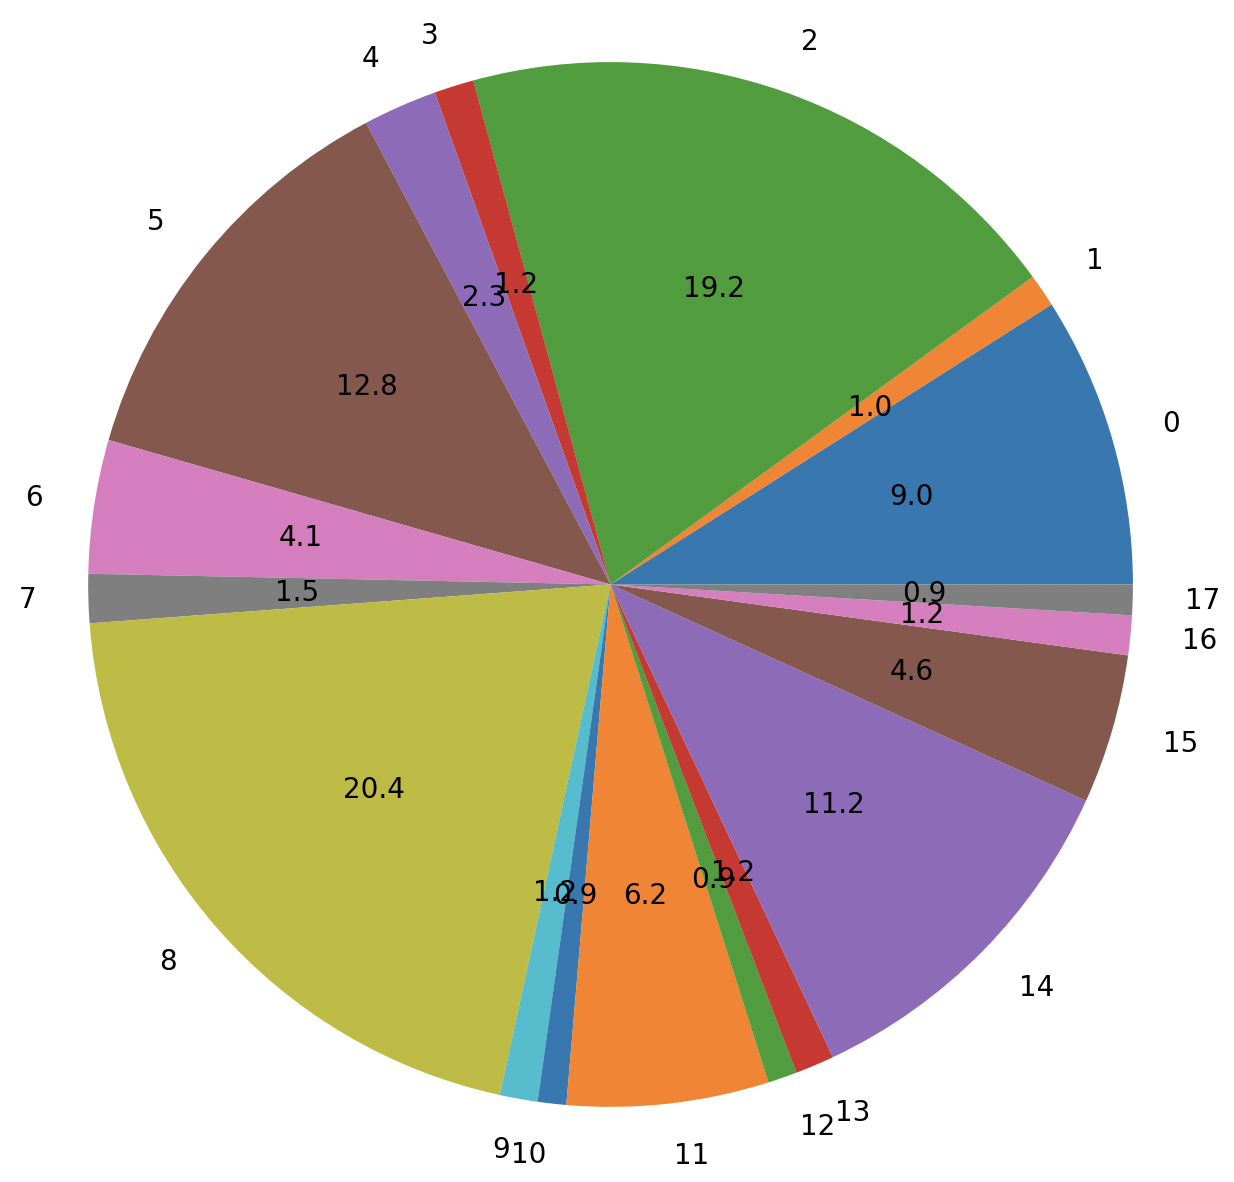
\includegraphics[width=0.8\columnwidth]{figures/dataExploration.png}
    \caption{Repartition of the classes in the train set (4888 proteins)}
    \label{fig:dataExploration}
\end{figure}

Another difficulty with our data is the small number of proteins in our dataset. In particular, state-of-the-art NLP techniques for computing representations from the sequences generally require much more massive data, of the order of a million data at least. This is why, for sequence-based embeddings, we used pretrained models from ProtTrans, that were trained on more that 393 billions amino acids \cite{protTrans}. 

The small size of our data was also problematic for structure-based embeddings. Indeed, the architectures we used (cf. section \ref{sec:structuralFeatures}) generally require more training data, and we found that all the GNNs we trained started to overfit from just a few tens of epochs. Again, data augmentation techniques exist for graphs \cite{Zhao2020}, but we did not implement them due to competition deadlines. 

To ensure that our models do not overfit on the input data, we split our initial train set of size 4888 into a train set of size 4644 (95\% of the data) and a validation set of size 244 (5\% of the data), containing at least one representative of each class. Those train and validation sets were perfectly identical for each of the models we trained, including the final SVC, to make sure that the performances we computed were accurate. 

\subsubsection{Data preprocessing}

The node features we had, stored in \texttt{node\_attributes.txt}, are represented in a table with 86 different features, some of them are numerical, and some of them are one hot encodings such as the columns from 4 to 23, which represent the 20 different amino acids. The attributes of the edges, stored in \texttt{edge\_attributes.txt}, contain the same type of features. Depending on their type, we have transformed the features as follows:
\begin{itemize}
    \item the one hot encoded features remained unchanged.
    \item numerical variables were scaled using the \texttt{StandardScaler} from \texttt{sklearn}
\end{itemize}

We used the DataLoader from \texttt{torch\_geometric.data}, to build the train, validation and test datasets in a specific shape with the following attributes: \texttt{x} : the nodes' features, \texttt{edge\_index}: representing all the edges from different graphs, \texttt{edge\_attr}: representing edge features, and finally \texttt{y} containing the target values.

\subsubsection{Computation resources and computation times}

For this competition, we only had access to limited computation resources, which forced us to focus on on moderate-sized architectures and pre-trained models.

Our CPU computations were done on a Intel Xeon W-1290P 3.70GHz with 10 physical cores. Our GPU computations were done on a NVIDIA GeForce RTX 3090 24Go.

\section{Our methods}

As explained above, our approach was done in three steps, which correspond to the sub-parts of this section: computing sequence-based embeddings, then structure-based embeddings, and eventually feeding a classifier with those embeddings.

\subsection{Sequence-based embeddings} \label{sec:sequentialFeatures}

In this section, we describe how we generated embeddings of our proteins using only the protein sequences, and not the graph structure. As explained before, protein sequence mining is equivalent to text mining on a dictionary of size 20, and this is why the techniques we describe in this section come from the NLP community.

\subsubsection{ProtTrans Embeddings}

Given the few data and computation resources we had access to, we decided to focus on Large Language Models (LLMs) pretrained on amino-acid sequences in an unsupervised setting. The most complete and easily accessible set of such models is probably ProtTrans \cite{protTrans}, so we decided to use it. More precisely, we used four pretrained models from ProtTrans: BERT (based on BERT architecture \cite{Bert2018}), BERT-BFD (same architecture, but trained on another dataset), ALBERT (based on ALBERT architecture \cite{Albert2019}), and XLNET (based on XLNet architecture \cite{XLNet2019}).

\paragraph{The truncation issue} The main limitation of those pretrained models is that, similarly to their corresponding NLP architectures, they only accept sequences of at most 512 tokens. This is a major issue for protein mining, since the sequences are often much larger than that. Some alternative architectures exist for long sequences, such as Big Bird \cite{bigBird2020}, however, to the best of our knowledge, no such architecture has been pretrained on amino-acid sequences, so we decided to use ProtTrans architecture with sequence truncation. Moreover, the truncation is not really problematic for us: over the 6,111 proteins we have, only 471 (7.7\%) are longer than 512, and the longest sequence is of size 989, so we can expect the beginning of the sequence to be informative enough to encapsulate the information we seek. 

\begin{figure}[h]
    \centering
    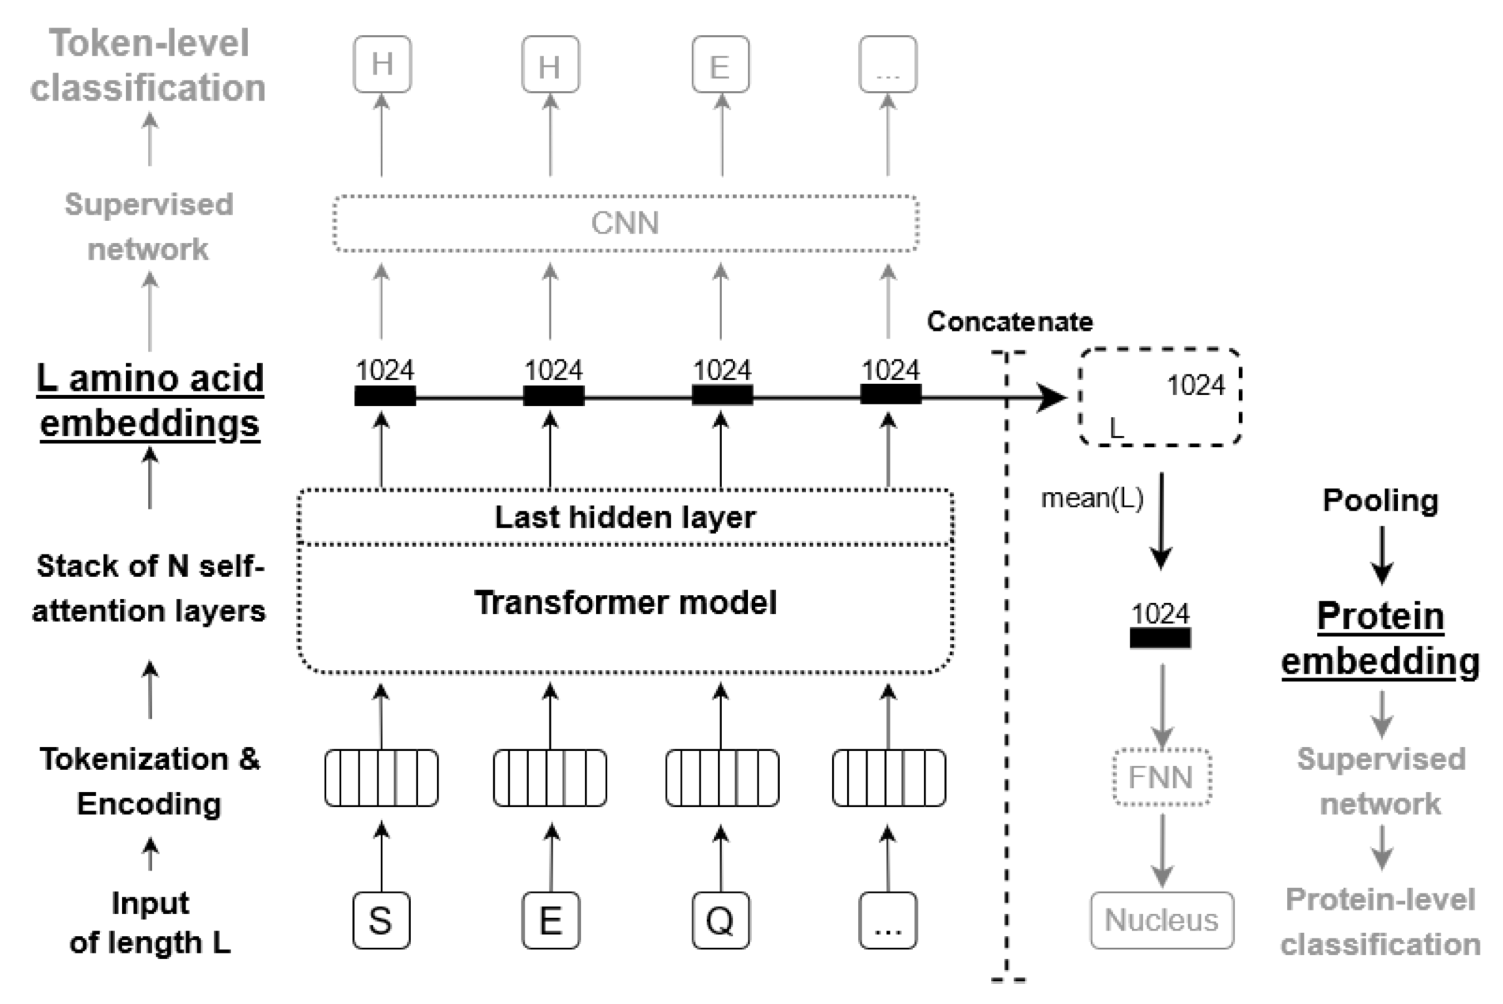
\includegraphics[width=\columnwidth]{figures/protbertTransformer.png}
    \caption{Feature extraction overview of ProtTrans models. Figure taken from \cite{protTrans}.}
    \label{fig:protTrans}
\end{figure}

\paragraph{ProtTrans model descriptions} Each of the four models we used (BERT, BERT-BFD, ALBERT, XLNet) is pretrained model on protein sequences using a Masked Language Modeling (MLM) objective. MLM is a self-supervised technique that avoid human labelling of the data, making it feasible to use enormous train sets. 

The idea is to extract the information learned by the protein LLM through embeddings, i.e., vector representations from the last hidden state of the protein model. In the transfer-learning step these embeddings served as input to subsequent supervised training. In our case however, we did not have the computation resources to fine tune each of those models on our classification task, so we directly computed the embeddings with the weights of the pretrained models, with no additional training.

\subsubsection{Tf-Idf embeddings}

Using Term Frequency-Inverse Document Frequency (TF-IDF) is quite common for feature extraction from text. This idea is pretty old (cf. \cite{SPARCKJONES1972} from 1972), but is still used today, such as in \cite{TFIDF}. The TF-IDF score of a word for a document in a collection of document represents the relevance of this word in this document compared to the others.

In our case, we chose all possible 4-grams of amino-acids that are present in every protein for dictionary. Then, our features are the TF-IDF score of each sequence of amino-acid for each token in this dictionary. 

\subsection{Structural features} \label{sec:structuralFeatures}

In this section, we describe how we generated embeddings of our proteins using only the protein structure. We recall that the protein structure data is represented as a graph with both node attributes and edge attributes. The nodes represent the amino acids and the edges encode relations between these nodes, in particular their 3D distance. Node attributes contain both positional features and features which characterize the amino acid chemical and biological properties.

We follow the general graph neural networks architecture, which starts by creating node level representations by leveraging different types of graph convolutions. We then aggregate these representations to form graph-level representations using readout layers. Most of the readout layers used in the literature can be implemented by simple operations, such as the sum, the mean or the max. 

\subsubsection{Architectures tested}

We used the Pytorch-Geometric (PyG) library, which makes it easy to train neural networks on graphs. For the results of each of those architectures, please refer to \ref{sec:results}.

We tested multiple architectures with different hyper-parameters which we manually tuned. Here's a list of the architectures that worked best. 

\paragraph{GCN}

The baseline model architecture, Graph Convolutional Network (GCN), apply linear operations on the node attributes and its neighborhood \ref{eq:GCN}. To avoid problems such as over-smoothing of the nodes attributes, we limit the number of successive graph convolutions to $4$.

\begin{equation} \label{eq:GCN}
    H^{k+1} = \sigma(\tilde{D} ^{-\frac{1}{2}}\tilde{A}  \tilde{D} ^{-\frac{1}{2}} H^k W^k), 
\end{equation}

where $W^k$ is a learned matrix, $\tilde{A}$ and $\tilde{D}$ are respectively the adjacency matrix and the degree matrix with added self-loops.

\paragraph{DGCNN}

Deep Graph Convolutional Neural Network (DGCNN, \cite{dgcnn}) has three sequential stages: (cf. figure \ref{fig:DGCNN})

\begin{itemize}
    \item The graph convolution layers extract vertices’ local substructure features and define a consistent vertex ordering
    \item A \texttt{SortPooling} layer sorts the vertex features under the previously defined order and unifies input sizes;
    \item The traditional convolutional and dense layers read the sorted graph representations and make predictions.
\end{itemize}

\begin{figure}[h]
    \centering
    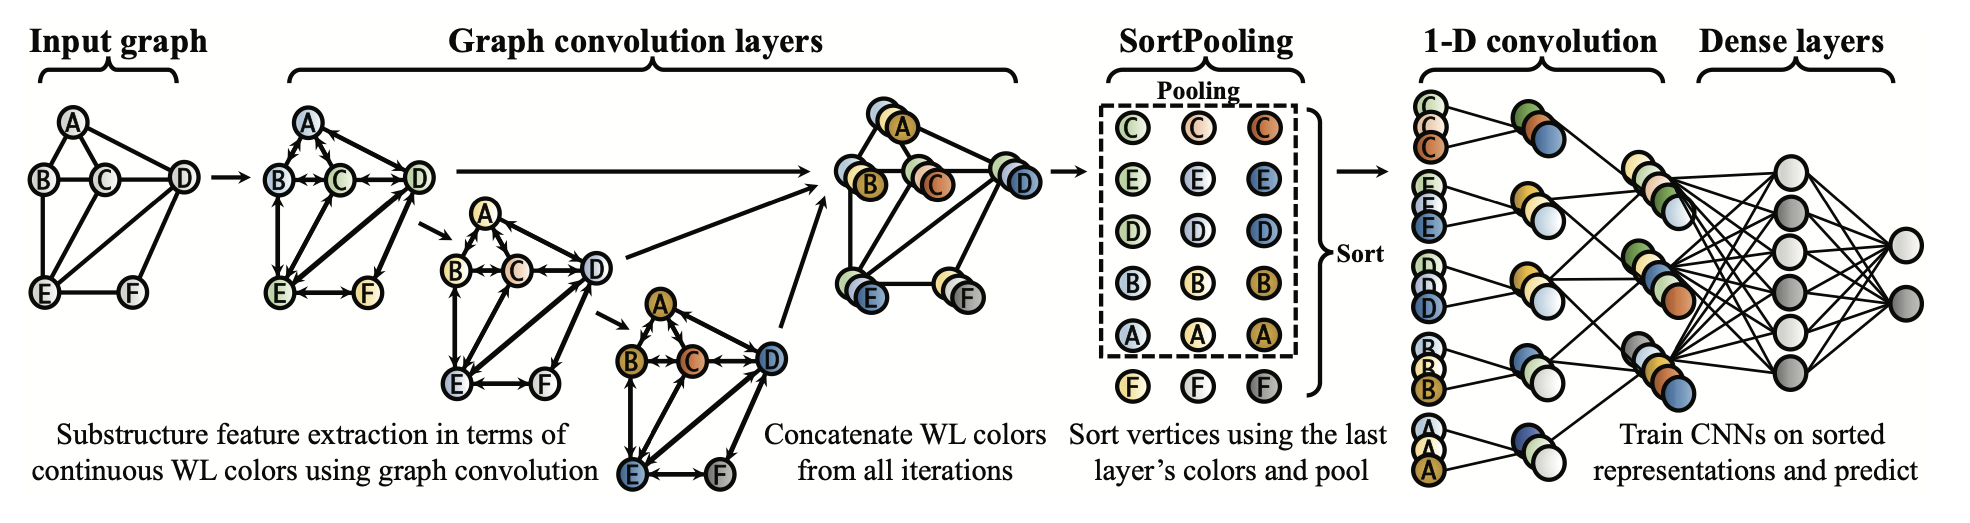
\includegraphics[width=\columnwidth]{figures/dgcnnArchitecture.png}
    \caption{DGCNN architecture. Figure taken from \cite{dgcnn}.}
    \label{fig:DGCNN}
\end{figure}

\paragraph{HGP}

Hierarchical Graph Pooling with Structure Learning (HGP-SL, \cite{hgp}) combines with Graph Neural Network, where graph pooling operations are added between graph convolution operations. It is composed of :

\begin{itemize}
    \item Graph pooling to induce subgraphs that preserve the informative nodes.
    \item Structure learning to learn the refined graph structure.
\end{itemize}

The advantage of this architecture is that it preserves the essential graph structure information for message passing procedure. The architecture allows learning graph representations in a hierarchical way based on the stacking of convolution and pooling operations. The readout function is used to summarize node representations at each level.

\begin{figure}[h]
    \centering
    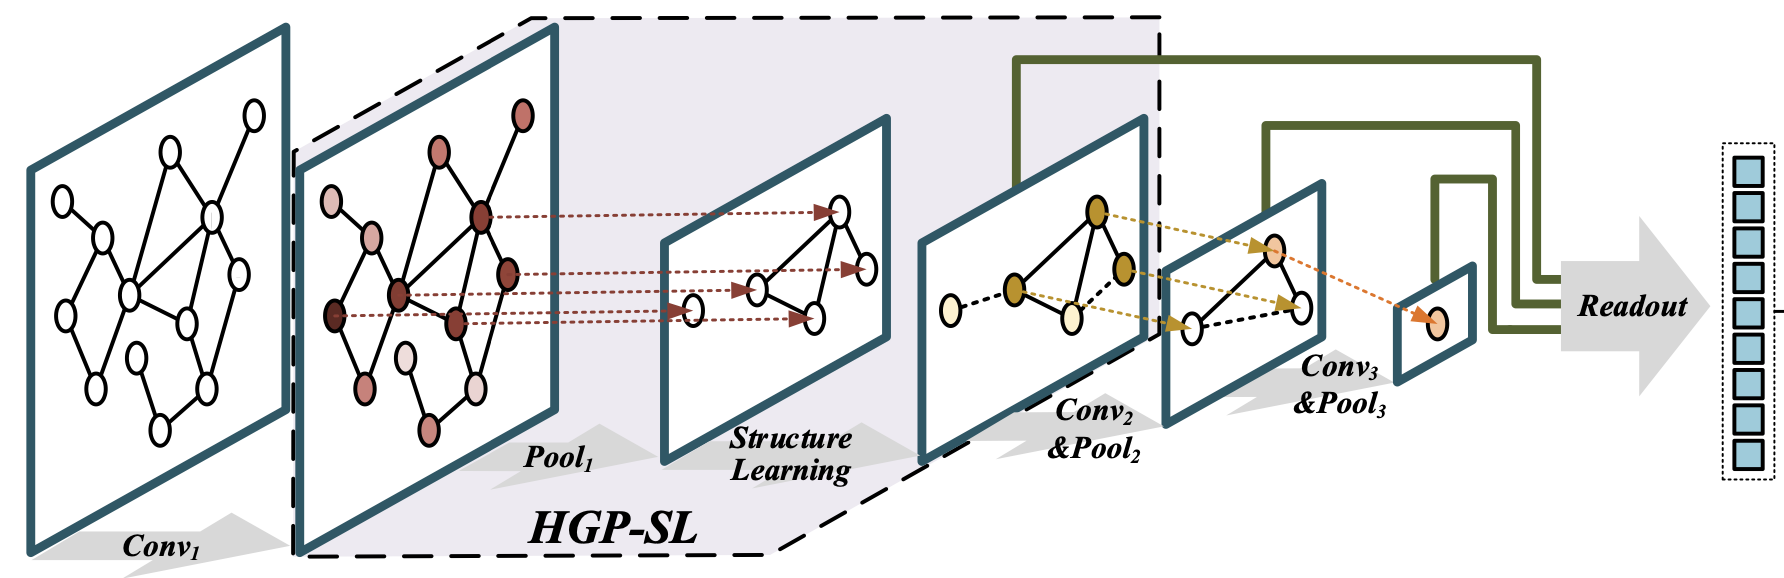
\includegraphics[scale=0.2]{figures/hgpArchitecture.png}
    \caption{Hierarchical Graph Pooling with Structure Learning. Figure taken from \cite{hgp}} 
    \label{fig:hdp}
\end{figure}

\paragraph{GAT}

Graph Attention networks (GAT, \cite{GAT}) are convolution-style neural networks that operate on graph-structured data, leveraging masked self-attentional layers.

This architecture uses efficient graph attention layers to assign different level of importance to different nodes within a neighborhood, while dealing with different sizes of neighborhoods. Furthermore, it does not depend on the knowledge of the entire graph structure upfront.

Additionally, it's one of the few graph architectures available with Pytorch Geometric, which allows the use of edge attributes, which are factored into the attention computation of each node. 

\begin{figure}[h]
    \centering
    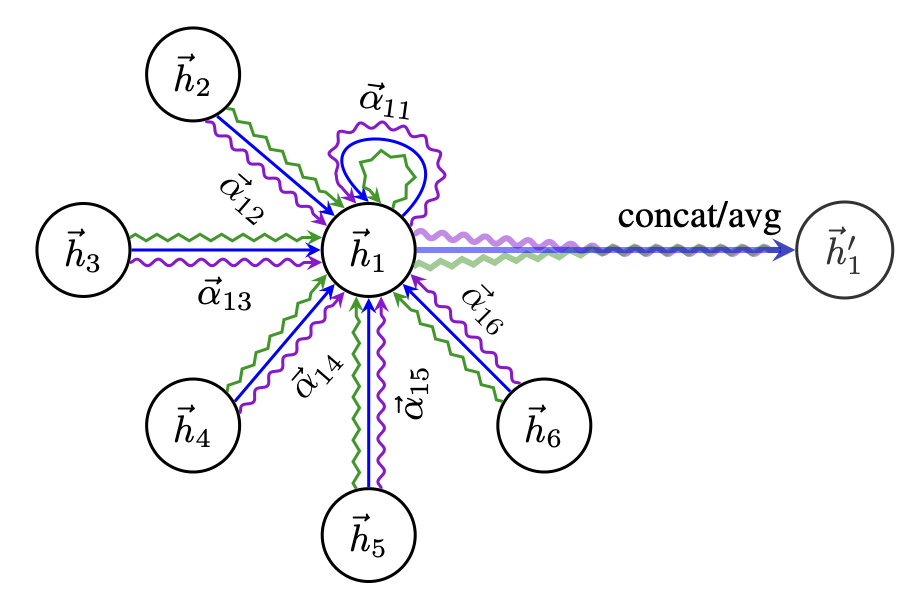
\includegraphics[width=0.8\columnwidth]{figures/attention.png}
    \caption{An illustration of multi-head attention (with K = 3 heads) by node 1 on its neighborhood. Figure taken from \cite{GAT}.}
    \label{fig:attention}
\end{figure}

\paragraph{GraphSAGE}

GraphSAGE \cite{graphsage} it is an inductive framework that leverages node attribute information to efficiently generate representations on previously unseen data. The core idea of this architecture is to sample and aggregate features from a node's neighborhood (cf. figure \ref{fig:graphSage}).

\begin{figure}[h]
    \centering
    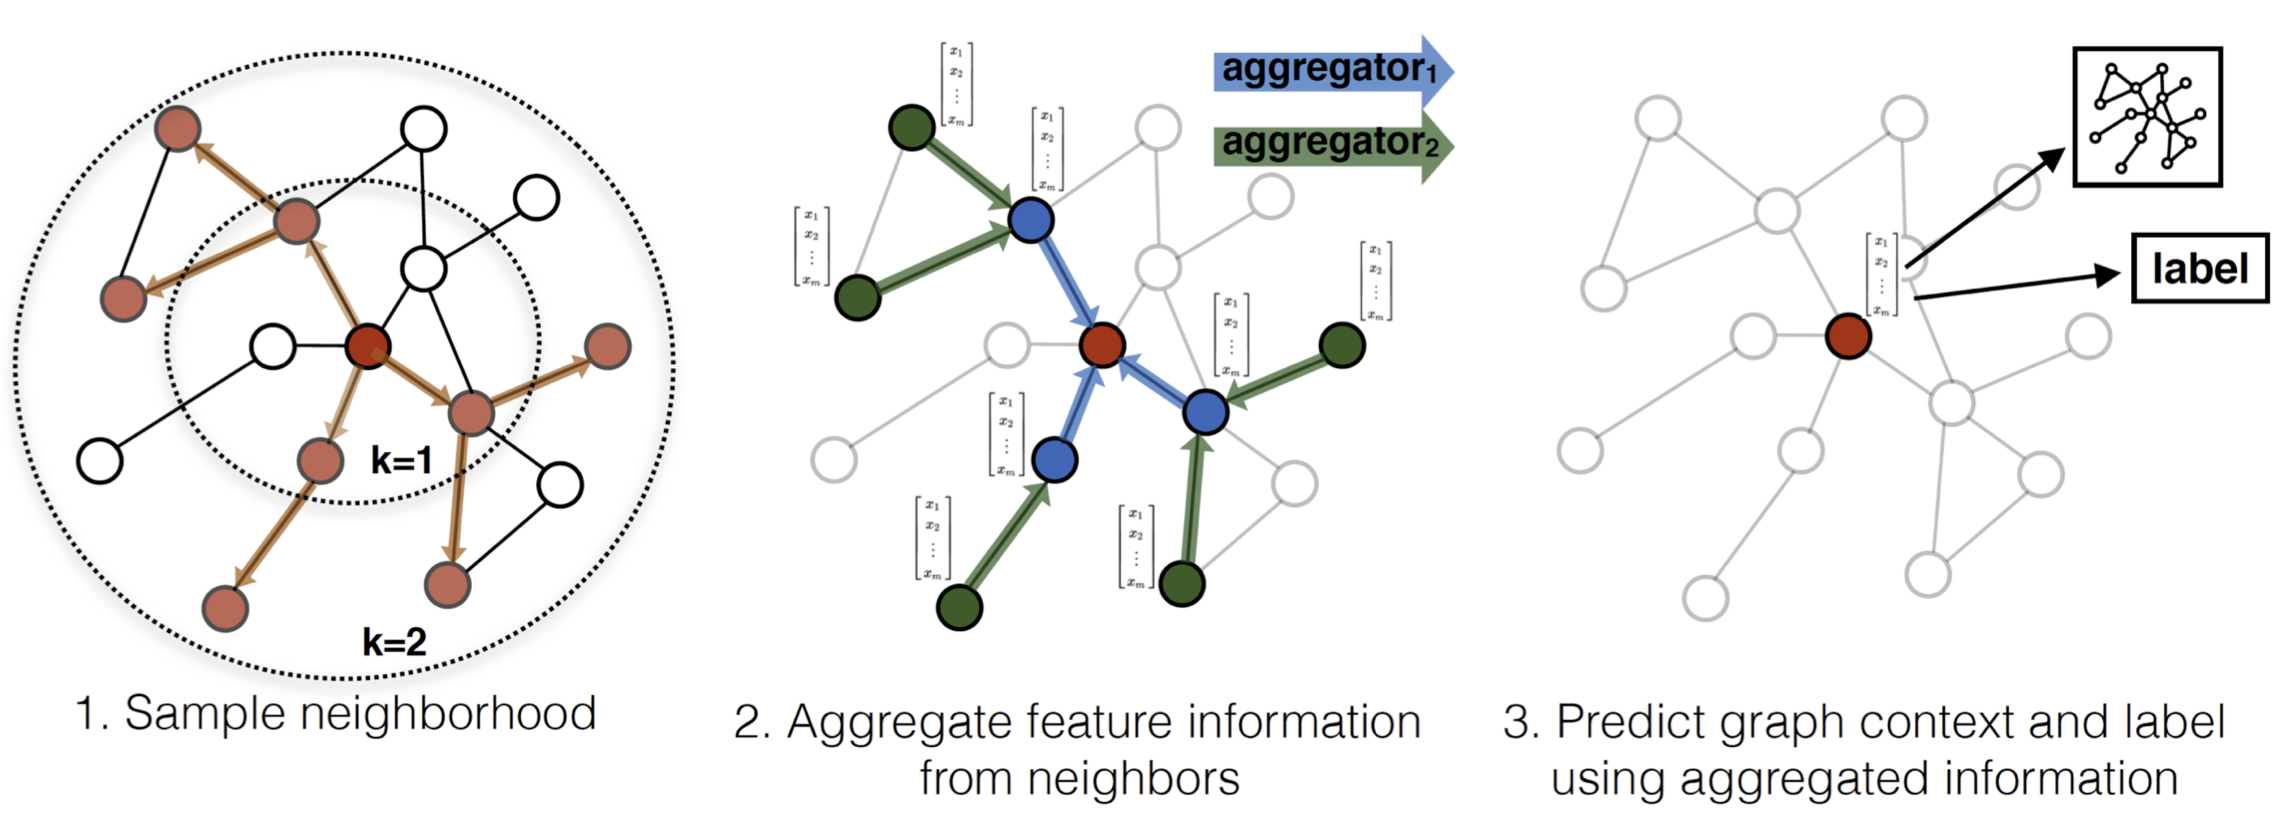
\includegraphics[width=\columnwidth]{figures/graphSageArchitecture.png}
    \caption{Visual illustration of the GraphSAGE sample and aggregate approach. Figure taken from \cite{graphsage}.}
    \label{fig:graphSage}
\end{figure}

\subsubsection{Architecture optimization}

In order to find the best parameters for our classification model, we studied the impact of the variation of some values on the results. We also compared different optimizers, mainly : \texttt{SGD}\texttt{Adam}, \texttt{AdamW} and \texttt{RSProp}. Among all of them, \texttt{Adam} optimizer performed best.

After studying the impact of the dropout rate on the results of the GAT and the HGP we fixed the value at 0.7. For the decay weight we fixed the value at $10^{-8}$.

We observed that our models were better performing with fewer features, so we first reduced the dimension of the nodes features using PCA, and we finally used features of dimension $13$ instead of $86$.

Moreover, to avoid overfitting, we evaluated our models on the train set at each epoch, and used early stopping with a patience parameter of 10 to stop the training and load the best model.

\subsection{Final classification} \label{sec:theClassifier}

As said before, we combined the embeddings we computed with various methods (cf. sections \ref{sec:sequentialFeatures}
 and \ref{sec:structuralFeatures}) in a classifier, to get the final classification.
 
\subsubsection{Choice of classifier}

In order to find the best classifier, we tested different ones for the classification prediction:

\begin{itemize}
    \item \texttt{KNeighborsClassifier}: it implements the k-nearest neighbors vote.
    \item \texttt{SVC}: Support Vector Classification
    \item \texttt{GaussianProcessClassifier}: it is based on Laplace approximation.
    \item \texttt{DecisionTreeClassifier}.
    \item \texttt{RandomForestClassifier}: it fits a number of decision tree classifiers on various sub-samples of the dataset and uses averaging to improve the predictive accuracy and control over-fitting.
    \item \texttt{MLPClassifier}: Multi-layer Perceptron classifier to optimize the log-loss function using LBFGS or stochastic gradient descent.
    \item \texttt{AdaBoostClassifier}: a meta-estimator that fits a classifier on the original dataset and then fits additional copies of the classifier on the same dataset but where the weights of incorrectly classified instances are adjusted such that subsequent classifiers.
\end{itemize} 

The best classifier in this case is the \texttt{SVC} with polynomial kernel, with parameters C equal to one (the penalty parameter of the error term given training vectors) and $\gamma$ equals to the inverse of the number of features (the coefficient for polynomial kernels). This is coherent with the survey \cite{surveyClassifProt}, which announced that SVC had one of the best performance for protein classification.

\subsubsection{Feature selection} \label{sec:featureSelection}

For the final classification, we had 10 embeddings for each proteins: 5 sequence-based (BERT, ALBERT, BERT-BFD, XLNet, and TF-IDF) and 5 structure-based (GNN, GDCNN, HGP, GraphSage, and GAT). This results in an enormous number of feature, which is not correctly handeled by the majority of classifiers. To reduce, the number of features, we did two things:

\begin{itemize}
    \item Using PCA for each type of embedding individually to reduce its length to at most 32. This is highly useful, since some embeddings are really long (1024 for the LLMs ones).
    \item Greedily optimizing to remove some embeddings and only keep the most informative ones (cf. below).
\end{itemize}

To select only the most informative set of embeddings, some advanced techniques exist, with strong theoretical foundations, such as using the mutual information between features to remove the redundant ones \cite{mutualInfo}. However, given the deadlines of the competitions, we did not implement such approaches, and we simply used greedy optimization: at each time, we add the embedding that improves the validation loss the most, until we do not observe any improvements (cf. table \ref{tab:performances}). Doing so, we finally selected only five embeddings: BERT, BERT-BFD, XLNet, GNN and DGCNN.

\begin{table}[h]
\centering
\begin{tabular}{|
>{\columncolor[HTML]{EFEFEF}}l |c|c|c|c|c|c|}
\hline
\textbf{Emb \textbackslash \ step} & \cellcolor[HTML]{EFEFEF}\textbf{1} & \cellcolor[HTML]{EFEFEF}\textbf{2} & \cellcolor[HTML]{EFEFEF}\textbf{3} & \cellcolor[HTML]{EFEFEF}\textbf{4} & \cellcolor[HTML]{EFEFEF}\textbf{5} & \cellcolor[HTML]{EFEFEF}\textbf{6} \\ \hline
\textbf{BERT} & \textbf{1.07} & - & - & - & - & - \\ \hline
\textbf{ALBERT} & 1.46 & NI & NI & NI & NI & NI \\ \hline
\textbf{BERT-BFD} & 1.13 & \textbf{0.97} & - & - & - & - \\ \hline
\textbf{XLNet} & 1.49 & 1.00 & \textbf{0.93} & - & - & - \\ \hline
\textbf{TF-IDF} & 2.43 & 1.07 & 0.96 & 0.93 & 0.90 & NI \\ \hline
\textbf{GNN} & 1.70 & 1.03 & 0.94 & \textbf{0.90} & - & - \\ \hline
\textbf{DGCNN} & 1.87 & 1.07 & NI & 0.92 & \textbf{0.89} & - \\ \hline
\textbf{HGP} & 1.95 & NI & NI & NI & NI & NI \\ \hline
\textbf{GraphSage} & 1.71 & NI & NI & 0.93 & 0.90 & NI \\ \hline
\textbf{GAT} & 1.98 & NI & NI & NI & NI & NI \\ \hline
\end{tabular}
\medskip 
\caption{Feature selection using the performances on the validation set and a greedy optimization. "NI" stands for "No Improvement", and at each step the embedding in bold is the selected one. The numbers corresponds to the log loss on the validation set.
\\ Lecture. At step 1, the most informative embedding was BERT, with a log-loss of 1.07, so it was selected. Then, adding other embeddings to BERT, ALBERT did not improved the performance of 1.07 (NI), and the most informative embedding was BERT-BFD with a performance of 0.97, so it was selected. This was continued untill no embeddings led to improvement.}
\label{tab:performances}
\end{table}

\section{Results and discussion} \label{sec:results}

\subsection{Results and computation times}

As shown in table \ref{tab:performances}, this approach led to a logarithmic loss of 0.89 on our validation set, which resulted in a public  score of 0.847 on Kaggle's leaderboard. The difference between those two numbers is probably linked to the small size of our validation set (244), which can have a huge impact on the loss, especially due to under-represented classes.

Using pretrained models and medium-size architecture for our graph neural networks, the computation time remained reasonable using NVIDIA GeForce RTX 3090 24Go as GPU: about 2h30 to compute the four embeddings of ProtTrans, few minutes for the TF-IDF embedding, and about 20min for the embeddings of all our graph models (for each of them, the training was early stopped after a few dozen of epochs to avoid overfitting).

Although we computed ten different embeddings for our proteins, in order to obtain the maximum performance we finally used only five of them for the final classification: three sequence-based embeddings, and two structure-based. The sequence-based embeddings appear to be much more useful for our classification task, even though the structure-based embeddings still improve the performance of the classification.

\subsection{Discussion}

 In this competition, we do not know exactly the source of the protein structure, but it appears that the sequence embeddings help the model classify way better than the graph approaches. This might be related to the protein structure data quality. It's possible that the protein structure data was only created based on the sequence data itself, using protein folding models for instance. Under this assumption, and despite the impressive accuracy rates of models like AlphaFold \cite{Jumper2021} on a number of tasks related to proteins (especially protein-protein interactions prediction), building and training graph models on top of that does not look promising, at least from our approach to this competition. 

 Compared to other graph tasks, graph classification literature isn't the most developed. Most approaches rely on other architectures that were created with a node-level or edge-level task in mind. The readout functions used are most of the time elementary which might be the main reason why these approaches are quite limited. One possible future development in this perspective is the use of trainable readout layers. 

\begin{comment}
\subsection{Standalone graph models results}
We first present the results we obtained with standalone graph neural networks that we tried. The numerical values refer to the negative log likelihood loss, obtained either on the training set or on the validation set, as described before. We also plot the time per epoch. As we use \textbf{early stopping} to avoid overtraining, it is more meaningful than using the overall training time. We show only the results we achieved after applying PCA to the node features, keeping only $13$ columns instead of $86$. 

\begin{table}[H]
\centering

 \begin{tabular}{||c || c  c  c||} 
  \hline
 Method & Train & Validation  & Time\\ [0.5ex] 
 \hline\hline
 Baseline & $1.07 \pm 0.03 $ & $1.86 \pm 0.02$ & 3 \\

 DGCNN & $1.85 \pm 0.05$ & $1.83 \pm 0.05$ & $1.5$\\

 HGP & & &\\

 GAT & $1.74 \pm 0.05$ & $1.85 \pm 0.05$  & $1.2$\\

 GAT (w/ edges) & $1.68 \pm 0.05$ & $1.83 \pm 0.05$ & $1.95$\\
 
 GrapheSAGE & $1.15 \pm 0.1$ & $1.82 \pm 0.05$  & $0.9$ \\ 

 \hline \hline

 \end{tabular}
\end{table}

\subsection{Final combination of embeddings}

We now show the results obtained for some combinations of sequence models, with or without using the graph embeddings, which were extracted from the last two layers of the best graph model (before the classification MLP head). We only show the scores obtained with the SVC classifier, which happened to have the best performance.

\begin{table}[H]
\centering

 \begin{tabular}{||c || c  c  c ||} 

\hline
 Method & Train & Validation & Time\\ [0.5ex] 
 \hline\hline
Bert + XLNet + Albert & & &\\

 \hline \hline
 \end{tabular}
\end{table}

One key takeaway from these results is that complex is not always necessarily better.
\end{comment}

\newpage
\printbibliography

\end{document}
